\documentclass{article}
\usepackage{tikz}
\usepackage{subfig}
\usepackage[margin=1.0in]{geometry}
\pagestyle{empty}
%\usepackage{framed}
\usepackage{pagecolor}
\usepackage{xcolor}


\begin{document}
%\newpagecolor{gray!40}
%\begin{framed}
N° USP:\\~\\
%\begin{center}\includegraphics[width=0.8\linewidth]{figs/digit_template}\end{center}
As respontas seguem a ordem das questões\\~\\
\fcolorbox{black}{white}{
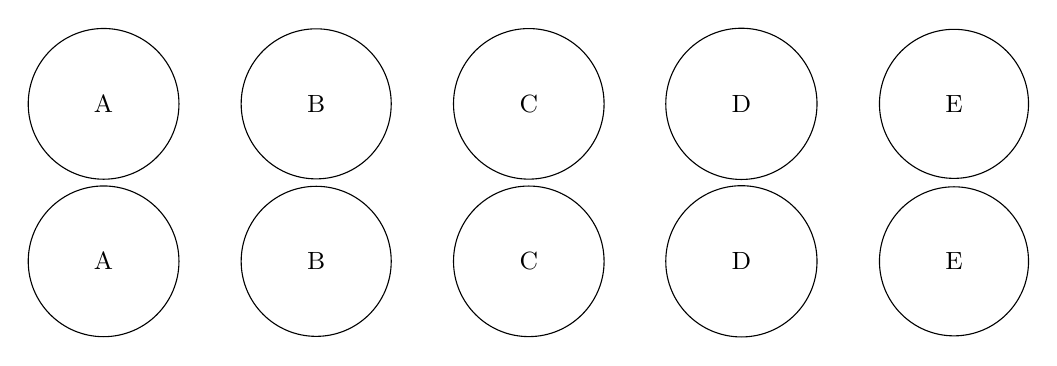
\begin{tikzpicture}[font=\small]
    \foreach \line in {1,2} {
        \begin{scope}[yshift=-2*\line cm]
            \foreach \letter/\position in {A/1, B/2, C/3, D/4, E/5} { 
                %\node at (0,0) {\normalsize\textbf{\line}};
                \node[draw,circle,inner sep=16pt] at ({\position * 2.7},0) {\letter};
            }
        \end{scope}
    }
\end{tikzpicture}\hfill
}
\\~\\
\\~\\
\\~\\
\\~\\
\\~\\
\\~\\
\\~\\
\\~\\
N° USP:\\~\\
%\begin{center}\includegraphics[width=0.8\linewidth]{figs/digit_template}\end{center}
As respontas seguem a ordem das questões\\~\\
\fcolorbox{black}{white}{
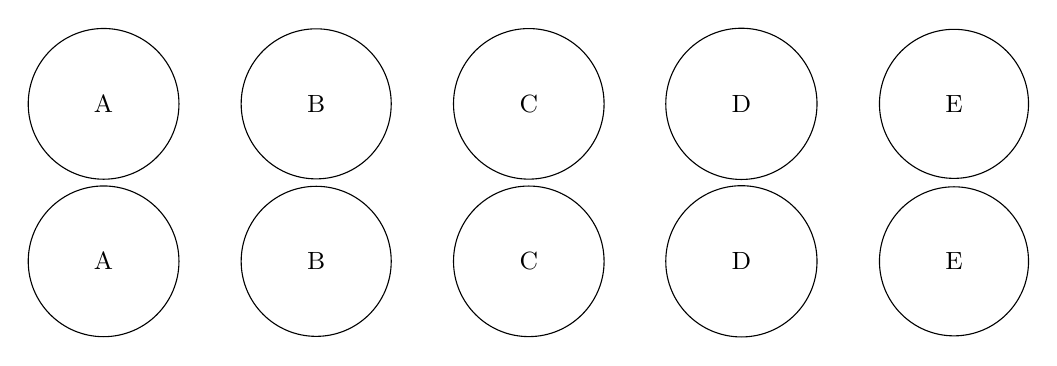
\begin{tikzpicture}[font=\small]
    \foreach \line in {1,2} {
        \begin{scope}[yshift=-2*\line cm]
            \foreach \letter/\position in {A/1, B/2, C/3, D/4, E/5} { 
                %\node at (0,0) {\normalsize\textbf{\line}};
                \node[draw,circle,inner sep=16pt] at ({\position * 2.7},0) {\letter};
            }
        \end{scope}
    }
\end{tikzpicture}\hfill
}
%\end{framed}
\end{document}